%%%%%%%%%%%%%%%%%%%%%%%%%%%%%%%%%%%%%%%%%%%%%%%%%%%%%%%%%%%%%%%%%%%%
%% I, the copyright holder of this work, release this work into the
%% public domain. This applies worldwide. In some countries this may
%% not be legally possible; if so: I grant anyone the right to use
%% this work for any purpose, without any conditions, unless such
%% conditions are required by law.
%%%%%%%%%%%%%%%%%%%%%%%%%%%%%%%%%%%%%%%%%%%%%%%%%%%%%%%%%%%%%%%%%%%%

\documentclass[
  digital,     %% The `digital` option enables the default options for the
               %% digital version of a document. Replace with `printed`
               %% to enable the default options for the printed version
               %% of a document.
%%  color,       %% Uncomment these lines (by removing the %% at the
%%               %% beginning) to use color in the printed version of your
%%               %% document
  oneside,     %% The `oneside` option enables one-sided typesetting,
               %% which is preferred if you are only going to submit a
               %% digital version of your thesis. Replace with `twoside`
               %% for double-sided typesetting if you are planning to
               %% also print your thesis. For double-sided typesetting,
               %% use at least 120 g/m² paper to prevent show-through.
  nosansbold,  %% The `nosansbold` option prevents the use of the
               %% sans-serif type face for bold text. Replace with
               %% `sansbold` to use sans-serif type face for bold text.
  nocolorbold, %% The `nocolorbold` option disables the usage of the
               %% blue color for bold text, instead using black. Replace
               %% with `colorbold` to use blue for bold text.         
  lof,         %% The `lof` option prints the List of Figures. Replace
               %% with `nolof` to hide the List of Figures.
  lot,         %% The `lot` option prints the List of Tables. Replace
               %% with `nolot` to hide the List of Tables.
]{fithesis4}

%% The following section sets up the locales used in the thesis.
\usepackage[resetfonts]{cmap} %% We need to load the T2A font encoding
\usepackage[T1,T2A]{fontenc}  %% to use the Cyrillic fonts with Russian texts.
\usepackage[main=english,
  english, czech, slovak
]{babel}
%%
%% The following section sets up the metadata of the thesis.
\thesissetup{
    date        = \the\year/\the\month/\the\day,
    university  = mu,
    faculty     = fi,
    department  = ,
    type        = prop,
    author      = Mgr. Filip Petrovič,
    gender      = m,
    advisor     = {prof. RNDr. Luděk Matyska},
    title       = {Autotuning and optimization of compute kernels},
    TeXtitle    = {Autotuning and optimization of compute kernels},
    keywords    = {autotuning, GPU optimization, CUDA, OpenCL},
    TeXkeywords = {autotuning, GPU optimization, CUDA, OpenCL},
    %% Remove the following line to use the JVS 2018 faculty logo.
    facultyLogo = fithesis-fi,
}

\usepackage{makeidx}      %% The `makeidx` package contains
\makeindex                %% helper commands for index typesetting.
%% These additional packages are used within the document:
\usepackage{paralist} %% Compact list environments
\usepackage{amsmath}  %% Mathematics
\usepackage{amsthm}
\usepackage{amsfonts}
\usepackage{url}      %% Hyperlinks
\usepackage{markdown} %% Lightweight markup
\usepackage{listings} %% Source code highlighting
\lstset{
  basicstyle      = \ttfamily,
  identifierstyle = \color{black},
  keywordstyle    = \color{blue},
  keywordstyle    = {[2]\color{cyan}},
  keywordstyle    = {[3]\color{olive}},
  stringstyle     = \color{teal},
  commentstyle    = \itshape\color{magenta},
  breaklines      = true,
}

\begin{document}

\chapter{Introduction}
In recent years, massively parallel devices such as modern CPUs and GPUs have become crucial in speeding up complex computations. These devices are used in areas such as physical simulations, weather forecasting, gaming, AI and many others. The speedup achieved by utilizing these devices can improve performance of these computations by several orders of magnitude. To employ these devices, a programmer needs to write code in a specialized language such as OpenCL or CUDA. The programs written in these languages are called compute kernels.

However, there is a portability issue with these kernels because devices are manufactured by different vendors and their architectures have distinct properties and performance. This means the kernel code must be tailored for a specific device. This process is time consuming because it is done by expert programmers who must optimize the computation manually. The issue can be solved by autotuning \cite{balaprakash2018autotuning} which is an optimization method that involves code parametrization to create multiple versions of computation. Each of these parameters affects code performance in a specific way and the aim of autotuning is to find a well-performing combination of these parameters that are fit to a device being utilized.

The autotuning can be introduced either manually or by using a framework. The second option makes it significantly easier to integrate autotuning in real-world applications. These frameworks contain many features that would be difficult to implement manually. There are several different ones available to choose from. Kernel Tuning Toolkit is a framework developed at Faculty of Informatics, Masaryk University in Brno. The aim of this thesis is to research and introduce several new features into this framework to make the autotuning more easier to use in practice.

\section{Thesis goals}
In this thesis, we focus on three main autotuning areas. They are the following ones:

\begin{itemize}
    \item Common autotuning format -- each of the autotuning frameworks has a specific programming API which is not portable. Certain APIs are not very well documented and can be quite complex to use. To solve this issue, we can create a high-level format to describe tuning problems. Next, we want to develop an application which can convert this format into framework-specific code. This will make it easier to port autotuned applications between different frameworks and make autotuning more accessible for programmers. Another benefit is that the format can be used in a benchmarking framework which compares performance of various autotuners and contains a shared database of autotuned code samples.
    \item Automatic tuning parameter generation -- currently, the tuning parameters need to be implemented by application developers, not by frameworks themselves. This can be rather difficult to achieve in more complex cases. It is possible to create a high-level language which generates certain common tuning parameters automatically. In this case, the tuning can be done transparently behind the scenes and programmer only needs to focus on writing application code. This can also make it easier for girls to write autotuning applications themselves. 
    \item Tuning space visualization -- it is difficult to imagine relations between different combinations of tuning parameters because the tuning output is only available in text form. It is possible to create an application which would visualize these relations which would help developers to find some hidden relationships between different parameters.
\end{itemize}

\chapter{Autotuning on parallel devices}

\section{Compute devices and APIs}
When we want to speed up a computation on parallel devices, we must write the code in a specialized language such as OpenCL or CUDA. Programs written in these languages are called compute kernels. OpenCL has an open API which is developed jointly by many companies and is supported on a wide range of devices (e.g., CPUs, GPUs, FPGAs, mobile devices). CUDA has a proprietary API developed by NVIDIA Corporation and it is focused mainly on GPUs made by NVIDIA. Both of these languages have similar programming model. An application is split into two parts -- a host application executed on a CPU and a kernel executed on a compute device. The host application is responsible for device management, memory management and kernel launching. The kernel usually contains the most computationally expensive part of application and that is why it executes many threads in parallel.

\subsection{Host application}
A host application is written in a regular language such as C or C++. It mostly handles inexpensive tasks such as data preparation, resource management and launching of compute kernels. OpenCL API defines the following structures which are needed to properly configure an OpenCL application:
\begin{itemize}
    \item \textit{Platform} -- An OpenCL platform represents an implementation of an OpenCL standard (e.g., a device driver developed by AMD, Intel or Nvidia).
    \item \textit{Device} -- Represents a specific compute device (e.g., AMD Ryzen 7 5800X, Nvidia GeForce RTX 3070). Devices are used for executing compute kernels.
    \item \textit{Context} -- A context holds all of the OpenCL runtime structures. It is akin to an operating system process. A context is created for a single OpenCL device and its lifetime is usually bound to an application runtime.
    \item \textit{Command queue} -- The commands such as launching of kernels and memory transfers are executed on an OpenCL device. These commands have to be submitted to a command queue where they are executed in a timely manner. It is possible to initialize multiple command queues within a single context to overlap independent operations.
    \item \textit{Buffer} -- Data accessed by a compute kernel have to be transferred into an OpenCL buffer. That is because kernels cannot directly acces the memory allocated by a host application. It is possible to specify a buffer memory location (device or host memory) and an access type (read and write access).
    \item \textit{Program} -- A program is compiled from an OpenCL C source file. Programs can be shared by multiple kernels so a single program has to be compiled only once.
    \item \textit{Kernel} -- Together, program and data create a compute kernel. The same compute kernel can be launched multiple times with different data.
    \item \textit{Event} -- Events serve as a synchronization primitive for individual commands submitted to a queue. It can also be used to retrieve information about a specific command such as computation status or duration.
\end{itemize}

An OpenCL application typically executes in the following phases:
\begin{enumerate}
    \item Platform and device selection
    \item Initialization of context and command queues
    \item Creation of memory buffers
    \item Program compilation and execution of a kernel function
    \item Transfer of data produced by a kernel from OpenCL buffers to host memory
\end{enumerate}

\subsection{Compute kernel}
Compute kernel is a function executed on a device. The kernel code is written from a perspective of a single \textit{work-item} which is the smallest OpenCL execution unit. Work-items operate in a lock-step mode so multiple work-items execute the same instruction on a different data in parallel. Each work-item has its own \textit{private memory} (i.e., the memory which is mapped to a CPU or a GPU register).

Work-items are organized into a larger structure which is \textit{work-group}. An OpenCL work-group can have up to three dimensions. The number and size of dimensions affects the amount of parallelism inside a kernel. The entire work-group is executed on a single \textit{compute unit} (e.g., a CPU core, a GPU streaming multiprocessor). It is possible for multiple work-groups to be executed on the same compute unit. On a work-group level, the work-items can access \textit{local memory} which is shared by all items belonging into the same group.

Individual work-groups are organized into \textit{NDRange} (N-Dimensional Range). At NDRange level, it is possible to address two types of memory -- \textit{global memory} and \textit{constant memory}. Global memory (e.g., CPU main memory, GPU global memory) is usually very large but has high latency. On the other hand, constant memory generally has a small capacity but lower latency. It can be utilized to store read-only data. Certain devices such as CPUs do not have hardware support for constant memory and usually store variables marked with constant memory keyword in global memory. Organization and indexing of work-groups inside an NDRange works in the same way as for work-items within a work-group. The entire hierarchy is illustrated in Figure \ref{opencl-hierarchy}.

\begin{figure}
    \begin{center}
    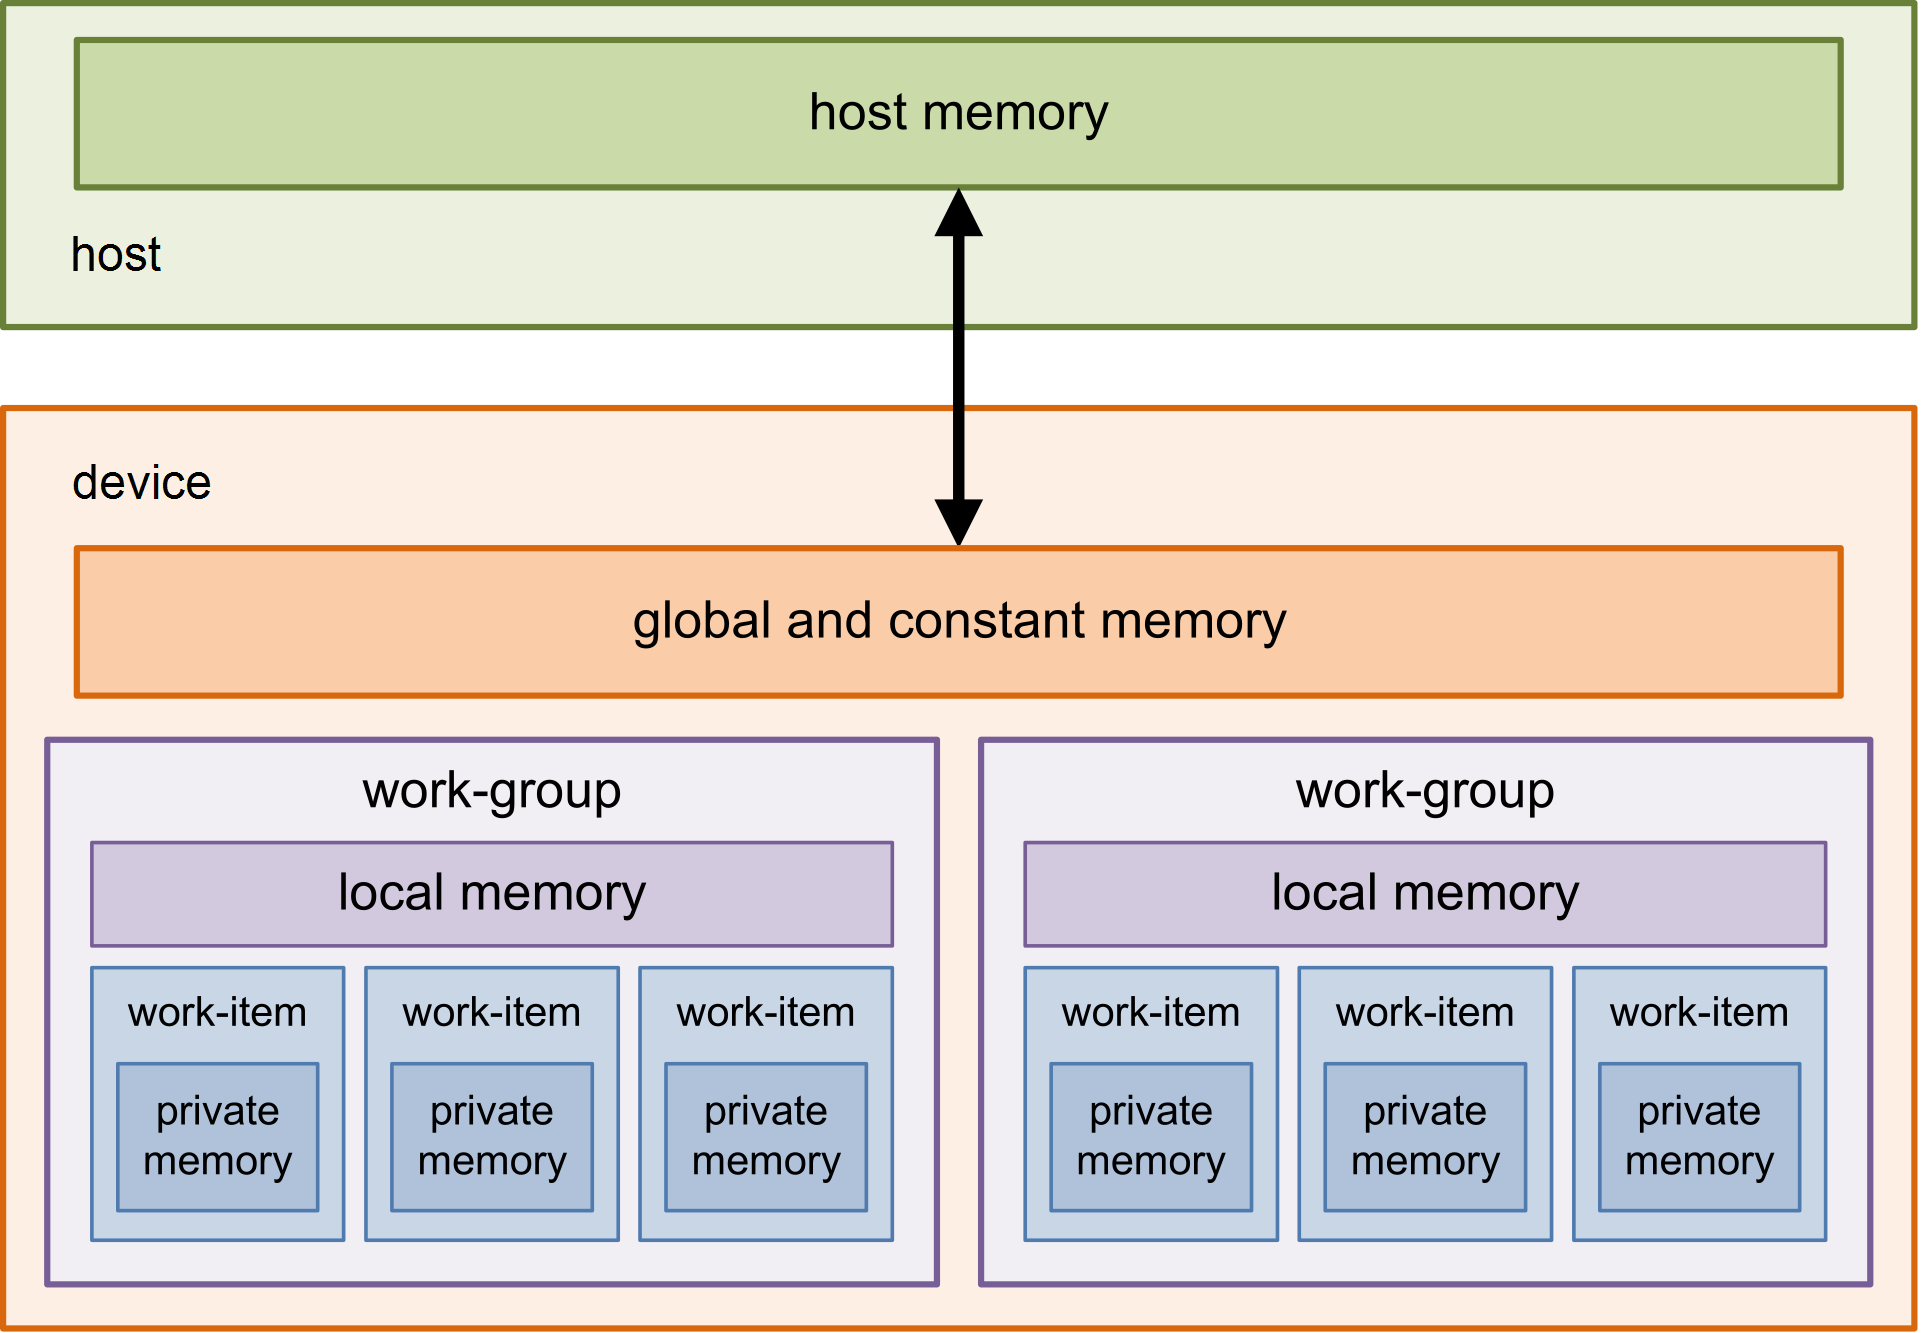
\includegraphics[width=125mm]{Figures/OpenClHierarchy.png}
    \end{center}
    \caption{OpenCL memory hierarchy, source: \cite{opencl-hierarchy-diagram}.}
    \label{opencl-hierarchy}
\end{figure}

\section{Autotuning}
Todo

\bibliographystyle{elsarticle-num}
\bibliography{ThesisProposal.bib}

\appendix %% Start the appendices.
\chapter{An appendix}
Here you can insert the appendices of your thesis.

\end{document}
